% Options for packages loaded elsewhere
\PassOptionsToPackage{unicode}{hyperref}
\PassOptionsToPackage{hyphens}{url}
%
\documentclass[
]{book}
\usepackage{lmodern}
\usepackage{amssymb,amsmath}
\usepackage{ifxetex,ifluatex}
\ifnum 0\ifxetex 1\fi\ifluatex 1\fi=0 % if pdftex
  \usepackage[T1]{fontenc}
  \usepackage[utf8]{inputenc}
  \usepackage{textcomp} % provide euro and other symbols
\else % if luatex or xetex
  \usepackage{unicode-math}
  \defaultfontfeatures{Scale=MatchLowercase}
  \defaultfontfeatures[\rmfamily]{Ligatures=TeX,Scale=1}
\fi
% Use upquote if available, for straight quotes in verbatim environments
\IfFileExists{upquote.sty}{\usepackage{upquote}}{}
\IfFileExists{microtype.sty}{% use microtype if available
  \usepackage[]{microtype}
  \UseMicrotypeSet[protrusion]{basicmath} % disable protrusion for tt fonts
}{}
\makeatletter
\@ifundefined{KOMAClassName}{% if non-KOMA class
  \IfFileExists{parskip.sty}{%
    \usepackage{parskip}
  }{% else
    \setlength{\parindent}{0pt}
    \setlength{\parskip}{6pt plus 2pt minus 1pt}}
}{% if KOMA class
  \KOMAoptions{parskip=half}}
\makeatother
\usepackage{xcolor}
\IfFileExists{xurl.sty}{\usepackage{xurl}}{} % add URL line breaks if available
\IfFileExists{bookmark.sty}{\usepackage{bookmark}}{\usepackage{hyperref}}
\hypersetup{
  pdftitle={NETISCE Manual and Tutorials},
  pdfauthor={Lauren Marazzi},
  hidelinks,
  pdfcreator={LaTeX via pandoc}}
\urlstyle{same} % disable monospaced font for URLs
\usepackage{color}
\usepackage{fancyvrb}
\newcommand{\VerbBar}{|}
\newcommand{\VERB}{\Verb[commandchars=\\\{\}]}
\DefineVerbatimEnvironment{Highlighting}{Verbatim}{commandchars=\\\{\}}
% Add ',fontsize=\small' for more characters per line
\usepackage{framed}
\definecolor{shadecolor}{RGB}{248,248,248}
\newenvironment{Shaded}{\begin{snugshade}}{\end{snugshade}}
\newcommand{\AlertTok}[1]{\textcolor[rgb]{0.94,0.16,0.16}{#1}}
\newcommand{\AnnotationTok}[1]{\textcolor[rgb]{0.56,0.35,0.01}{\textbf{\textit{#1}}}}
\newcommand{\AttributeTok}[1]{\textcolor[rgb]{0.77,0.63,0.00}{#1}}
\newcommand{\BaseNTok}[1]{\textcolor[rgb]{0.00,0.00,0.81}{#1}}
\newcommand{\BuiltInTok}[1]{#1}
\newcommand{\CharTok}[1]{\textcolor[rgb]{0.31,0.60,0.02}{#1}}
\newcommand{\CommentTok}[1]{\textcolor[rgb]{0.56,0.35,0.01}{\textit{#1}}}
\newcommand{\CommentVarTok}[1]{\textcolor[rgb]{0.56,0.35,0.01}{\textbf{\textit{#1}}}}
\newcommand{\ConstantTok}[1]{\textcolor[rgb]{0.00,0.00,0.00}{#1}}
\newcommand{\ControlFlowTok}[1]{\textcolor[rgb]{0.13,0.29,0.53}{\textbf{#1}}}
\newcommand{\DataTypeTok}[1]{\textcolor[rgb]{0.13,0.29,0.53}{#1}}
\newcommand{\DecValTok}[1]{\textcolor[rgb]{0.00,0.00,0.81}{#1}}
\newcommand{\DocumentationTok}[1]{\textcolor[rgb]{0.56,0.35,0.01}{\textbf{\textit{#1}}}}
\newcommand{\ErrorTok}[1]{\textcolor[rgb]{0.64,0.00,0.00}{\textbf{#1}}}
\newcommand{\ExtensionTok}[1]{#1}
\newcommand{\FloatTok}[1]{\textcolor[rgb]{0.00,0.00,0.81}{#1}}
\newcommand{\FunctionTok}[1]{\textcolor[rgb]{0.00,0.00,0.00}{#1}}
\newcommand{\ImportTok}[1]{#1}
\newcommand{\InformationTok}[1]{\textcolor[rgb]{0.56,0.35,0.01}{\textbf{\textit{#1}}}}
\newcommand{\KeywordTok}[1]{\textcolor[rgb]{0.13,0.29,0.53}{\textbf{#1}}}
\newcommand{\NormalTok}[1]{#1}
\newcommand{\OperatorTok}[1]{\textcolor[rgb]{0.81,0.36,0.00}{\textbf{#1}}}
\newcommand{\OtherTok}[1]{\textcolor[rgb]{0.56,0.35,0.01}{#1}}
\newcommand{\PreprocessorTok}[1]{\textcolor[rgb]{0.56,0.35,0.01}{\textit{#1}}}
\newcommand{\RegionMarkerTok}[1]{#1}
\newcommand{\SpecialCharTok}[1]{\textcolor[rgb]{0.00,0.00,0.00}{#1}}
\newcommand{\SpecialStringTok}[1]{\textcolor[rgb]{0.31,0.60,0.02}{#1}}
\newcommand{\StringTok}[1]{\textcolor[rgb]{0.31,0.60,0.02}{#1}}
\newcommand{\VariableTok}[1]{\textcolor[rgb]{0.00,0.00,0.00}{#1}}
\newcommand{\VerbatimStringTok}[1]{\textcolor[rgb]{0.31,0.60,0.02}{#1}}
\newcommand{\WarningTok}[1]{\textcolor[rgb]{0.56,0.35,0.01}{\textbf{\textit{#1}}}}
\usepackage{longtable,booktabs}
% Correct order of tables after \paragraph or \subparagraph
\usepackage{etoolbox}
\makeatletter
\patchcmd\longtable{\par}{\if@noskipsec\mbox{}\fi\par}{}{}
\makeatother
% Allow footnotes in longtable head/foot
\IfFileExists{footnotehyper.sty}{\usepackage{footnotehyper}}{\usepackage{footnote}}
\makesavenoteenv{longtable}
\usepackage{graphicx,grffile}
\makeatletter
\def\maxwidth{\ifdim\Gin@nat@width>\linewidth\linewidth\else\Gin@nat@width\fi}
\def\maxheight{\ifdim\Gin@nat@height>\textheight\textheight\else\Gin@nat@height\fi}
\makeatother
% Scale images if necessary, so that they will not overflow the page
% margins by default, and it is still possible to overwrite the defaults
% using explicit options in \includegraphics[width, height, ...]{}
\setkeys{Gin}{width=\maxwidth,height=\maxheight,keepaspectratio}
% Set default figure placement to htbp
\makeatletter
\def\fps@figure{htbp}
\makeatother
\setlength{\emergencystretch}{3em} % prevent overfull lines
\providecommand{\tightlist}{%
  \setlength{\itemsep}{0pt}\setlength{\parskip}{0pt}}
\setcounter{secnumdepth}{5}
\usepackage{booktabs}
\usepackage[]{natbib}
\bibliographystyle{plainnat}

\title{NETISCE Manual and Tutorials}
\author{Lauren Marazzi}
\date{2021-12-08}

\usepackage{amsthm}
\newtheorem{theorem}{Theorem}[chapter]
\newtheorem{lemma}{Lemma}[chapter]
\newtheorem{corollary}{Corollary}[chapter]
\newtheorem{proposition}{Proposition}[chapter]
\newtheorem{conjecture}{Conjecture}[chapter]
\theoremstyle{definition}
\newtheorem{definition}{Definition}[chapter]
\theoremstyle{definition}
\newtheorem{example}{Example}[chapter]
\theoremstyle{definition}
\newtheorem{exercise}{Exercise}[chapter]
\theoremstyle{definition}
\newtheorem{hypothesis}{Hypothesis}[chapter]
\theoremstyle{remark}
\newtheorem*{remark}{Remark}
\newtheorem*{solution}{Solution}
\begin{document}
\maketitle

{
\setcounter{tocdepth}{1}
\tableofcontents
}
\hypertarget{about}{%
\chapter{About}\label{about}}

Welcome to the NETISCE manual and tutorials.

NETISCE is a workflow that identified control node perturbations for cellular reprogramming. This manual contains directions for intial setup, as well as tutorials for reproducing NETISCE cell reprogramming results in developmental, stem cell, and cancer biology.

\hypertarget{installation-and-usage}{%
\chapter{Installation and Usage}\label{installation-and-usage}}

\hypertarget{download-netisce}{%
\section{Download NETISCE}\label{download-netisce}}

NETISCE pipelines can be downloaded from our github repository: \url{https://github.com/veraliconaresearchgroup/netisce}

We recommend that you run NETISCE on a high-performance cluster (hpc), as you may generate files that are quite large, or run computations that may take a long time. However, we provide two Nextflow pipelines, one designed for hpcs \href{https://github.com/VeraLiconaResearchGroup/Netisce/tree/main/NETICSE_hpc}{(NETISCE\_hpc)}, and another for running NETISCE on a local machine \href{https://github.com/VeraLiconaResearchGroup/Netisce/tree/main/NETICSE_local}{(NETISCE\_local)}.

\hypertarget{install-nextflow}{%
\section{Install Nextflow}\label{install-nextflow}}

Nextflow is required to run the NETISCE pipeline. Please follow the instructions from \url{https://www.nextflow.io/} (see `Getting Started' steps 1 \& 2) to install Nextflow in the appropriate NETSICE folder (\_local or \_hpc).

\hypertarget{docker-image}{%
\section{Docker Image}\label{docker-image}}

\emph{docker image provided here TBD}

\hypertarget{prerequisuites}{%
\section{Prerequisuites}\label{prerequisuites}}

If you are not using the Docker image, the following packages will need to be installed:

\begin{itemize}
\tightlist
\item
  \href{https://scipy.org/install/}{scipy}
\item
  \href{https://pandas.pydata.org/getting_started.html}{pandas}
\item
  \href{https://scikit-learn.org/stable/install.html}{sklearn}
\item
  \href{https://www.scikit-yb.org/en/latest/quickstart.html}{yellowbrick}
\end{itemize}

\hypertarget{params}{%
\section{Parameters and Configuration}\label{params}}

Whether on your local machine or hpc, to run NETISCE you must specify the files and parameters within the \texttt{.nf} file

\begin{itemize}
\tightlist
\item
  \textbf{params.expressions}: csv file containing normalized expression data for network nodes in different samples
\item
  \textbf{params.network}: network file (sif format)
\item
  \textbf{params.samples}: text file specifying the phenotype for each sample in params.expressions file (tab delimited)
\item
  \textbf{params.internal\_control}: text file containing a list of nodes to be used as internal marker nodes
\item
  \textbf{params.alpha}: alpha parameter for signal flow analysis (default =0.9)
\item
  \textbf{params.undesired}: string of the undesired phenotype (as labeled in the params.samples file)
\item
  \textbf{params.desired}: string of the desired phenotype (as labeled in the params.samples file)
\item
  \textbf{params.filter}: filtering parameter for criterion 2 (``strict'' or ``relaxed'')
\item
  \textbf{params.kmeans\_min\_val}: minimum k-means value for clustering (default=2)
\item
  \textbf{params.kmeans\_max\_val}: maximum k-means value for clustering (default=10)
\item
  \textbf{params.num\_nodes}: number of nodes in network for which normalized expression data exists (within the params.expressions file)
\item
  \textbf{params.num\_states}: number of randomly generated initial states (default=100000, or 3\^{}n where n is the number of network nodes and 3\^{}n is less than 100000)
\end{itemize}

Please see the \textbf{input\_data} folder for examples of files to match the formatting.

\hypertarget{netisce_mutations.nf}{%
\subsection{NETISCE\_mutations.nf}\label{netisce_mutations.nf}}

If you are interested in including mutational information, please use the \texttt{NETISCE\_mutations.nf} pipeline. You must additionally specify \texttt{params.mutations}: a csv file containing mutational configuration for network nodes (0 for loss of function, 1 for gain of function). Please see example in \texttt{input\_data} for formatting.

\hypertarget{nextflow.config}{%
\subsection{nextflow.config}\label{nextflow.config}}

If you are running nextflow on an hpc, please specify your executor, and clusterOptions within the nextflow.config file. Please see \url{https://www.nextflow.io/docs/latest/config.html} for more information regarding your executor.

\hypertarget{running-netisce}{%
\section{Running NETISCE}\label{running-netisce}}

Once you have specified the parameters, run NETSICE using the following command:

\begin{verbatim}
./nextflow run NETISCE.nf -resume ##or NETISCE_mutations.nf if including mutational data
\end{verbatim}

We recommend using the -resume flag in the case that you change a file or parameter within your pipeline. This way, nextflow caches results that remain unchanged, preventing pipeline steps from being re-run.

\hypertarget{netsice-output}{%
\chapter{NETSICE output}\label{netsice-output}}

After the NETISCE computations are complete, the output files will be located in the \texttt{results} folder. Please note that we have included in this folder the most relevant output files that you may want to use for further analysis. However, you can explore all outputs by checking within each step of the pipeline's work folder.

The contents of each file are briefly described below. For more details and to see example outputs, please see the \protect\hyperlink{toy}{Toy Network Examples}.

\hypertarget{section-id}{%
\subsubsection*{exp\_internalmarkers.txt}\label{section-id}}
\addcontentsline{toc}{subsubsection}{exp\_internalmarkers.txt}

This file contains the resultant steady state values for the internal marker nodes for the provided experimental samples (those specified in samples.txt) from Signal Flow Analysis.

\hypertarget{section-id}{%
\subsubsection*{experimental\_internalmarkers.pdf}\label{section-id}}
\addcontentsline{toc}{subsubsection}{experimental\_internalmarkers.pdf}

This pdf is a figure of the steady state values for the internal marker nodes for the provided experimental samples. This can be used to verify the validity of the internal marker nodes.

\hypertarget{section-id}{%
\subsubsection*{elbow.png}\label{section-id}}
\addcontentsline{toc}{subsubsection}{elbow.png}

A graph of the elbow metric for determining the optimal k for k-means.

\hypertarget{section-id}{%
\subsubsection*{silhouette.pdf}\label{section-id}}
\addcontentsline{toc}{subsubsection}{silhouette.pdf}

A graph of the silhouette metric for determining the optimal k for k-means.

\hypertarget{section-id}{%
\subsubsection*{fvs.txt}\label{section-id}}
\addcontentsline{toc}{subsubsection}{fvs.txt}

This file contains the node names for the FVS used as control nodes for the NETISCE run.

\hypertarget{section-id}{%
\subsubsection*{crit1perts.txt}\label{section-id}}
\addcontentsline{toc}{subsubsection}{crit1perts.txt}

This file contains a list of IDs for the control node perturbations that passed criterion 1.

\hypertarget{section-id}{%
\subsubsection*{pert1\_internal\_markers.txt}\label{section-id}}
\addcontentsline{toc}{subsubsection}{pert1\_internal\_markers.txt}

This file contains a table of the internal marker node steady state values from control node perturbations whose associated attractors passed the first filtering criterion.

\hypertarget{section-id}{%
\subsubsection*{successful\_controlnode\_perturbations.txt}\label{section-id}}
\addcontentsline{toc}{subsubsection}{successful\_controlnode\_perturbations.txt}

This file contains a table of the control node perturbations that pass both the 1st and 2nd filtering criteria. it also contains the number of upregulation,downregulations, and total number of nodes perturbed for each perturbation set.

\hypertarget{toy}{%
\chapter{Toy Network Examples}\label{toy}}

Here, we will walk through a brief tutorial of a NETISCE run. The files necessary to complete the tutorial are within the \texttt{input\ data} folder of both \href{https://github.com/VeraLiconaResearchGroup/Netisce/tree/main/NETICSE_local}{\texttt{NETISCE\_local}} and \href{https://github.com/VeraLiconaResearchGroup/Netisce/tree/main/NETICSE_hpc}{\texttt{NETISCE\_hpc}}.
The results from these Toy examples can be found in the \href{https://github.com/VeraLiconaResearchGroup/Netisce/tree/main/toy_example_results}{toy\_example\_results} folder of the main github repository.

\hypertarget{overview}{%
\section{Overview}\label{overview}}

We will use a simple toy network of 6 nodes and 9 edges.

\begin{figure}

{\centering 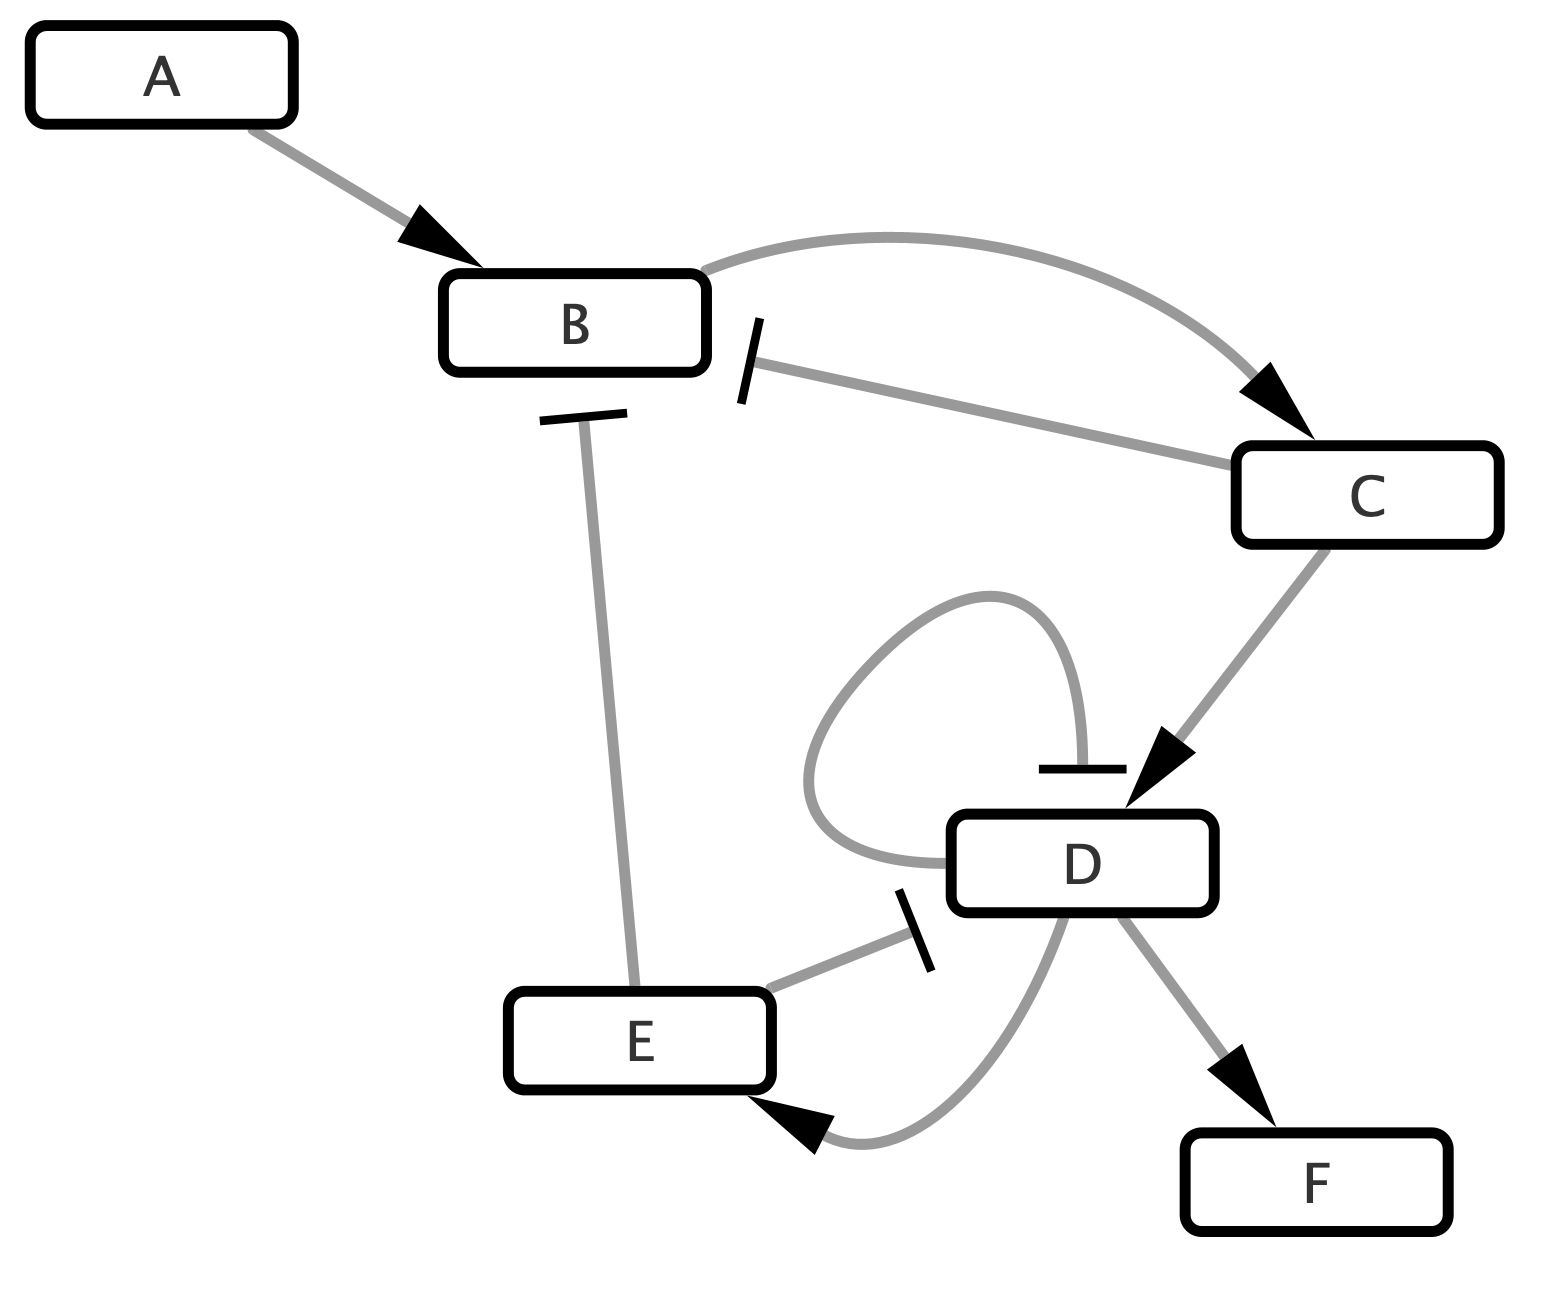
\includegraphics[width=0.5\linewidth]{images/toy_network} 

}

\caption{Simple Toy Network}\label{fig:unnamed-chunk-2}
\end{figure}

\hypertarget{data}{%
\section{Data}\label{data}}

You can find the relevant data files in the \texttt{input\_data} folder.

In this example, we have 2 samples, A and B, with three replicates each (A\_1,A\_2,A\_3, etc).
The normalized expression data is housed in \texttt{expressions.csv}, and contains normalized expression values for 4 of the network nodes (in this case, node C was not found to be expressed in the samples).

\begin{tabular}{l|r|r|r|r|r|r}
\hline
X & A\_1 & A\_2 & A\_3 & B\_1 & B\_2 & B\_3\\
\hline
A & 2 & 1 & 2 & 6 & 7 & 6\\
\hline
B & 6 & 7 & 6 & 2 & 1 & 1\\
\hline
D & -1 & -1 & -2 & 6 & 7 & 6\\
\hline
E & 2 & 1 & 2 & 6 & 7 & 6\\
\hline
\end{tabular}

The \texttt{samples.txt} file specifies that A is associated to a treatment sensitive phenotype, while B is associated to a resistance phenotype.

\begin{tabular}{l|l}
\hline
name & phenotype\\
\hline
A\_1 & sensitive\\
\hline
A\_2 & sensitive\\
\hline
A\_3 & sensitive\\
\hline
B\_1 & resistant\\
\hline
B\_2 & resistant\\
\hline
B\_3 & resistant\\
\hline
\end{tabular}

Note that you can use any term to describe the phenotypes. Just be sure to be consistent with the \texttt{param.desried} and \texttt{param.undesired} variables within the Nextflow \texttt{.nf} file.

Lastly, we need to include a list of internal marker nodes. This list is in \texttt{internal\_marker.txt}. For our small network, the internal marker node is \texttt{C}.

\begin{tabular}{l}
\hline
C\\


\hline
\end{tabular}

\hypertarget{netisce-run-configuration}{%
\section{NETISCE run configuration}\label{netisce-run-configuration}}

With all your input data files loaded, next we configure the nextflow run.
Within either \texttt{NETISCE\_local} or \texttt{NETSICE\_hpc} (\textbf{Note: while we do recommend you run NETISCE on a hpc, this example is small enough to run locally}).

Open up \texttt{NETISCE.nf}. Here, you need to specify the parameters for the Nextflow run on lines 3-19. Please refer to \protect\hyperlink{params}{section 2.5} for parameter definitions.

For this example, your parameters should look like:

\begin{verbatim}
params.expressions = "$baseDir/input_data/expressions.csv"
params.network = "$baseDir/input_data/network.sif"
params.samples = "$baseDir/input_data/samples.txt"
params.internal_control="$baseDir/input_data/internal_marker.txt"
params.alpha = 0.9
params.undesired = 'resistant'
params.desired = 'sensitive'
params.filter ="strict"


params.kmeans_min_val = 2
params.kmeans_max_val = 10


params.num_nodes = 4 // that have expression data
params.num_states = 1000
\end{verbatim}

\textbf{Some Notes: } make sure to include \texttt{\$baseDir} before pointing to the folder containing your input data. Also, be sure that \texttt{params.num\_nodes} is the number of nodes where there exists normalized expression data within \texttt{expression.csv}. Finally, in \texttt{NETISCE.nf}, mutations are not considered, so that like is commented out.

\hypertarget{run-netsice}{%
\section{Run NETSICE}\label{run-netsice}}

In your terminal/command prompt, navigate to the appropriate NETISCE folder \texttt{\_hpc} or \texttt{local}. To start your run, enter \texttt{./nextflow\ run\ NETISCE.nf\ -resume}.
While NETISCE is running, your terminal should look like this, where you can see the progress on each step of the pipeline:

\begin{figure}

{\centering 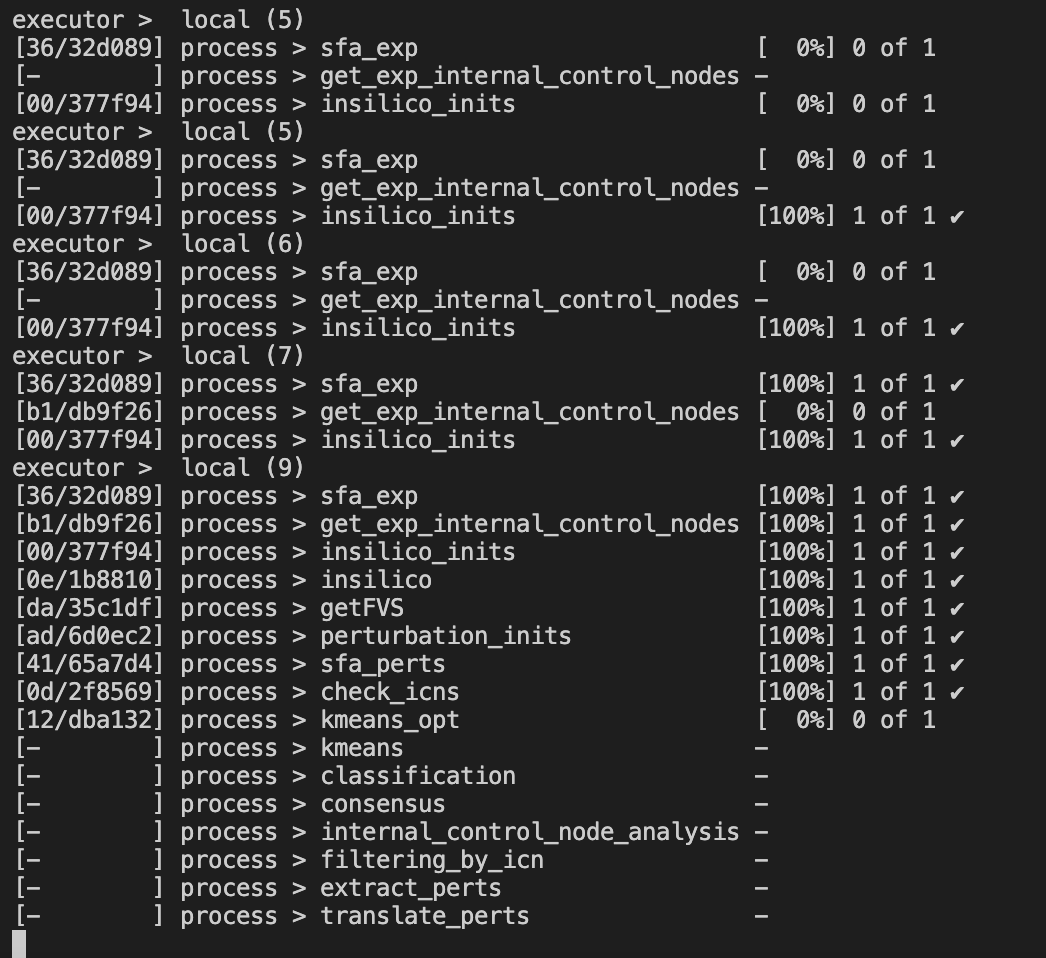
\includegraphics[width=0.5\linewidth]{images/running_shot} 

}

\caption{Terminal when running NETISCE}\label{fig:unnamed-chunk-6}
\end{figure}

Once the run has successfully completed, the process will end and the following will be displayed:

\begin{figure}

{\centering 
\includegraphics[width=0.5\linewidth]{images/completed} 

}

\caption{Terminal when running NETISCE}\label{fig:unnamed-chunk-7}
\end{figure}

\hypertarget{netsice-results}{%
\section{NETSICE Results}\label{netsice-results}}

Let's take a look at the results of our NETISCE run, where the goal was to shift the system from the undesired state B, and towards the desired state A. These results can be found in the toy\_example\_1 subfolder of the \href{https://github.com/VeraLiconaResearchGroup/Netisce/tree/main/toy_example_results}{toy\_example\_results} folder of the main github repository.

\hypertarget{section-id}{%
\subsubsection*{exp\_internalmarkers.txt}\label{section-id}}
\addcontentsline{toc}{subsubsection}{exp\_internalmarkers.txt}

Our internal marker node was node C. In this file we see the steady state values of the node in the A and B sample replicates (the output values from SFA).

\begin{tabular}{l|r}
\hline
name & C\\
\hline
A\_1 & 0.4278056\\
\hline
A\_2 & 0.4802943\\
\hline
A\_3 & 0.4361991\\
\hline
B\_1 & 0.1590962\\
\hline
B\_2 & 0.0982107\\
\hline
B\_3 & 0.0935476\\
\hline
\end{tabular}

\hypertarget{section-id}{%
\subsubsection*{experimental\_internalmarkers.pdf}\label{section-id}}
\addcontentsline{toc}{subsubsection}{experimental\_internalmarkers.pdf}

The above numbers may be a little challenging to read! So, we have included a plot of the values in the\texttt{experimental\_internalmarkers.pdf}:

\begin{figure}

{\centering 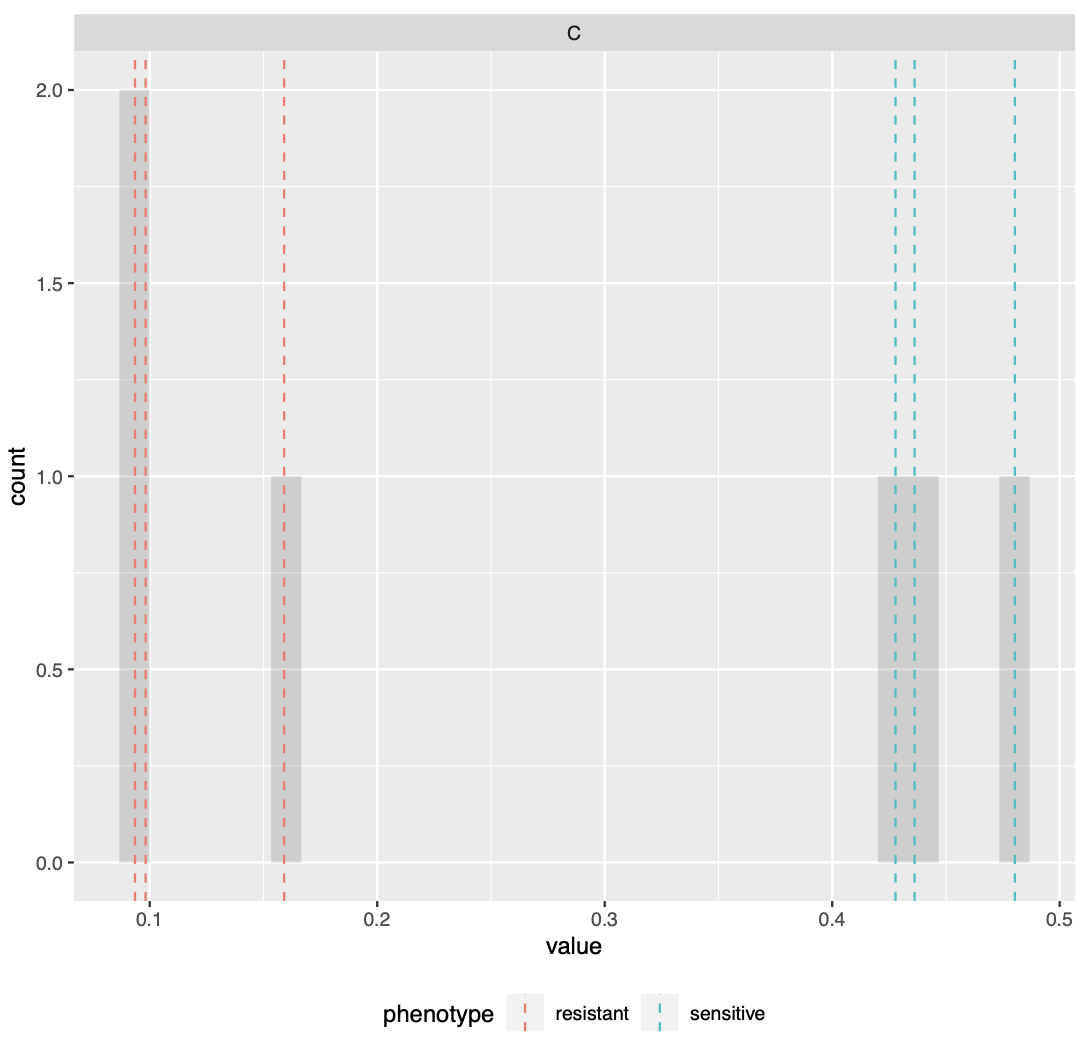
\includegraphics[width=0.5\linewidth]{images/expmarkers} 

}

\caption{experimental marker node steady state values}\label{fig:unnamed-chunk-9}
\end{figure}

On this histogram, we see bars for each of the samples and their replicates. The A (sensitive) samples are marked by a blue vertical line at their steady state value, while the B (resistant) samples are marked by a red vertical line at their steady state value. Here, we see that the values of node C are well separated between the two phenotypes (all of the A values are greater than all of the B values). We will assume that this also aligns with the biological knowledge of the system.

In this example, since there are only 4 network nodes that have normalized expression values, NETISCE generates the maximum number of random initial states, \(3^4\), or 81.

After estimating attractors for the experimental and randomly generated initial states, the resultant attractors were clustered using k-means clustering. The elbow and silhouette metrics are used to determine the optimal number k.

\hypertarget{section-id}{%
\subsubsection*{elbow.png}\label{section-id}}
\addcontentsline{toc}{subsubsection}{elbow.png}

\begin{figure}

{\centering 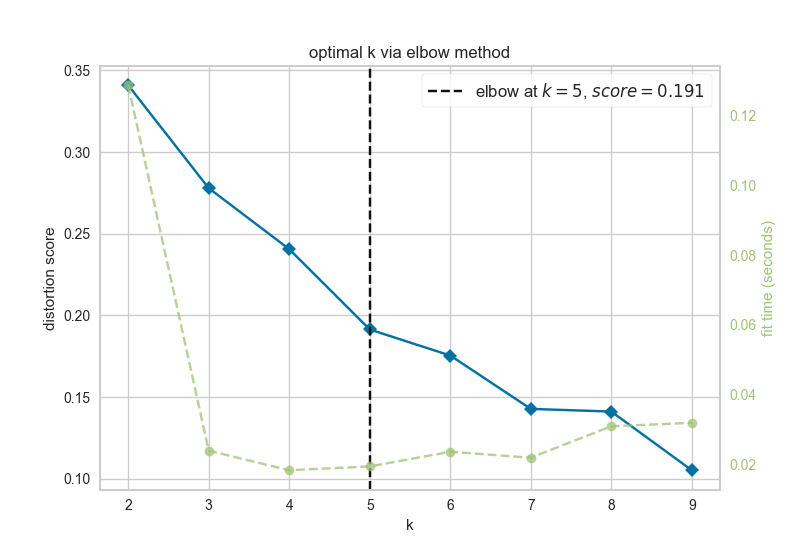
\includegraphics[width=0.5\linewidth]{results/elbow} 

}

\caption{elbow metric for optimal k}\label{fig:unnamed-chunk-10}
\end{figure}

The elbow metric found the optimal number of k clusters to be k=4.

\hypertarget{section-id}{%
\subsubsection*{silhouette.pdf}\label{section-id}}
\addcontentsline{toc}{subsubsection}{silhouette.pdf}

\begin{figure}

{\centering 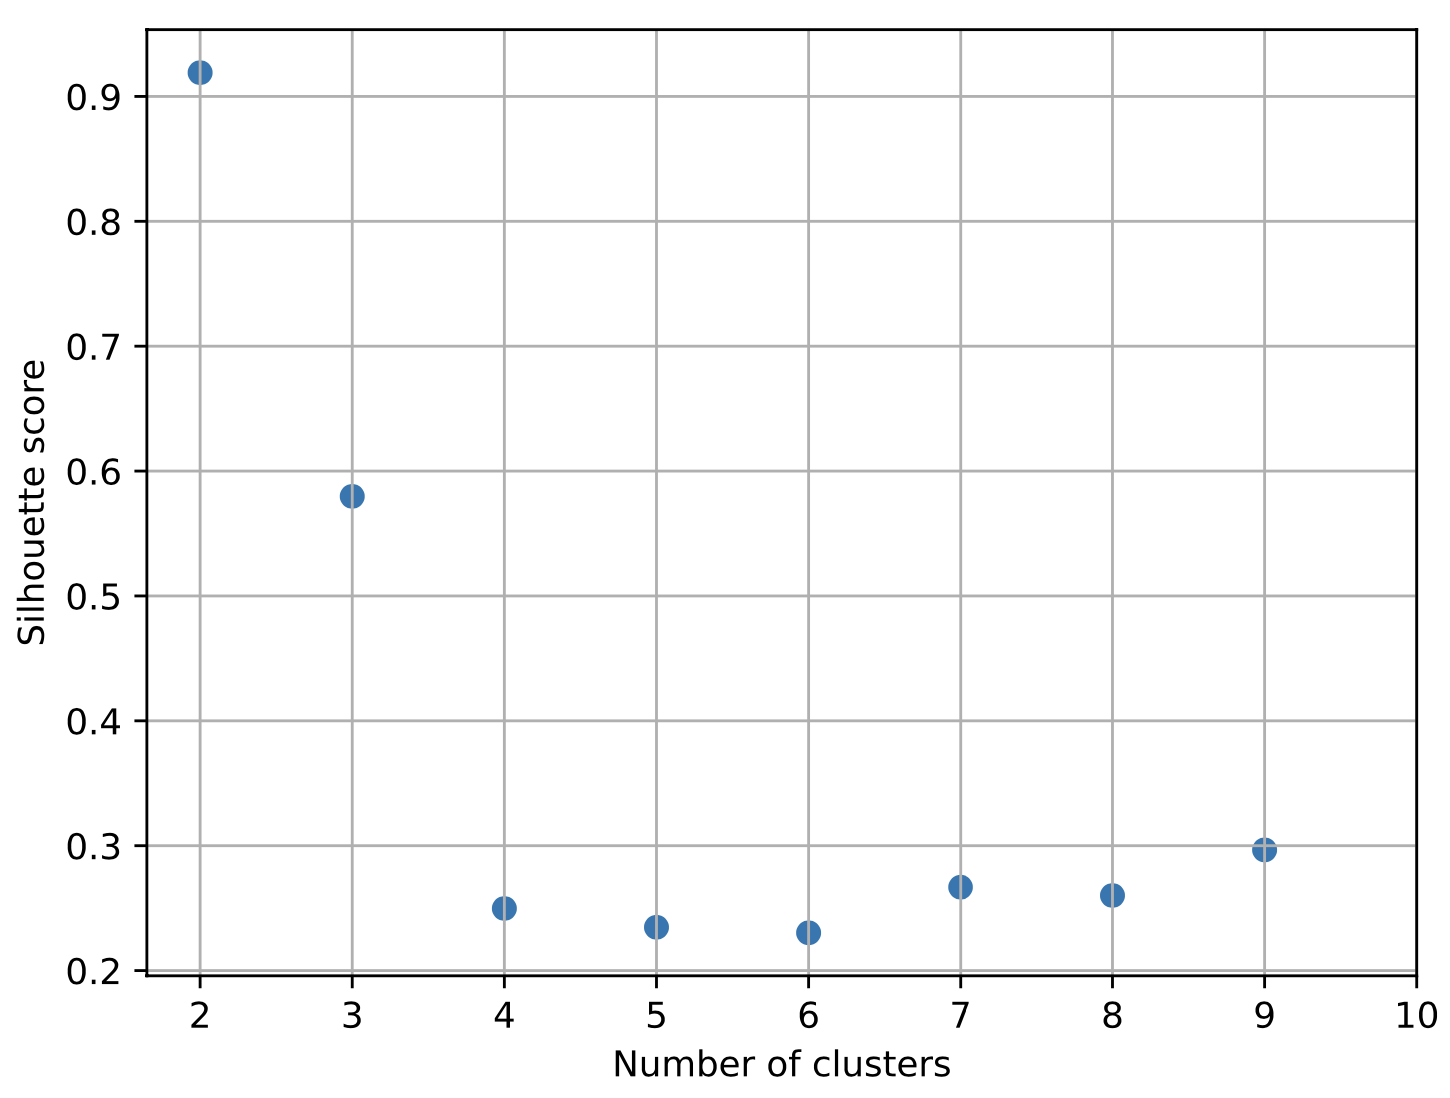
\includegraphics[width=0.5\linewidth]{images/silhouette} 

}

\caption{silhouette metric for optimal k}\label{fig:unnamed-chunk-11}
\end{figure}

The silhouette metric found the optimal number of k clusters to be k=2.

Since the optimal ks identified by the silhouette metric and the elbow metric do not match, NETISCE chooses the smaller k, as long as the phenotypes remain separate (NETISCE checks to make sure this is true).

\hypertarget{section-id}{%
\subsubsection*{fvs.txt}\label{section-id}}
\addcontentsline{toc}{subsubsection}{fvs.txt}

This file contains the node names that were identified by the FVS finding algorithm.

\begin{tabular}{l}
\hline
name\\
\hline
D\\
\hline
B\\
\hline
\end{tabular}

The FVS finding algorithm identified nodes B and D to be the minimal FVS control nodes in the toy network. Since the FVS control node set contained 2 nodes, 9 combinations of perturbations were performed on the control node sets.

\hypertarget{section-id}{%
\subsubsection*{crit1perts.txt}\label{section-id}}
\addcontentsline{toc}{subsubsection}{crit1perts.txt}

This file contains a list of IDs for the perturbations to FVS control nodes that passed criterion 1.

\begin{tabular}{l}
\hline
V1\\
\hline
pert\_0\\
\hline
pert\_1\\
\hline
pert\_2\\
\hline
pert\_4\\
\hline
pert\_5\\
\hline
pert\_6\\
\hline
pert\_7\\
\hline
pert\_8\\
\hline
\end{tabular}

8 out of the 9 pertrubations passed the machine learning filtering criterion.

\hypertarget{section-id}{%
\subsubsection*{pert1\_internal\_markers.txt}\label{section-id}}
\addcontentsline{toc}{subsubsection}{pert1\_internal\_markers.txt}

This file contains a table of the internal marker node state values from control node perturbations whose associated attractors passed the first filtering criterion.

\begin{tabular}{l|r}
\hline
name & C\\
\hline
pert\_0 & -2.7000000\\
\hline
pert\_1 & 1.0209997\\
\hline
pert\_2 & 6.3000000\\
\hline
pert\_4 & -0.0427445\\
\hline
pert\_5 & 6.3000000\\
\hline
pert\_6 & -2.7000000\\
\hline
pert\_7 & -2.8528056\\
\hline
pert\_8 & 6.3000000\\
\hline
\end{tabular}

\hypertarget{section-id}{%
\subsubsection*{successful\_controlnode\_perturbations.txt}\label{section-id}}
\addcontentsline{toc}{subsubsection}{successful\_controlnode\_perturbations.txt}

This file contains a table of the perturbations on FVS control nodes that passed both the 1st and 2nd filtering criteria. it also contains the number of upregulation,downregulations, and total number of nodes perturbed for each perturbation set.

\begin{tabular}{l|l|l|r|r|r}
\hline
  & D & B & up & down & total\\
\hline
pert\_1 & down & nochange & 0 & 1 & 1\\
\hline
pert\_5 & nochange & up & 1 & 0 & 1\\
\hline
pert\_2 & down & up & 1 & 1 & 2\\
\hline
pert\_8 & up & up & 2 & 0 & 2\\
\hline
\end{tabular}

Here, we see that four perturbations that passed both filtering criteria.

Let's take a quick look at the steady state values for these perturbations, and the attractors generated from the experimental data:

\begin{tabular}{l|l|r}
\hline
  & name & C\\
\hline
1 & A\_1 & 0.4278056\\
\hline
2 & A\_2 & 0.4802943\\
\hline
3 & A\_3 & 0.4361991\\
\hline
4 & B\_1 & 0.1590962\\
\hline
5 & B\_2 & 0.0982107\\
\hline
6 & B\_3 & 0.0935476\\
\hline
21 & pert\_1 & 1.0209997\\
\hline
31 & pert\_2 & 6.3000000\\
\hline
51 & pert\_5 & 6.3000000\\
\hline
8 & pert\_8 & 6.3000000\\
\hline
\end{tabular}

Indeed, we see that the steady-state expression values of node C in the attractors generated by peturbations to the FVS control nodes are all are greater than the steady-state expression values of node C in the attractors generated from the sensitive A sample. A successful reprogramming from resistant (B) to sensitive (A) cells has occurred!

\hypertarget{toy-example-with-mutations}{%
\section{Toy Example with mutations}\label{toy-example-with-mutations}}

Let's say that in our system, gene A exhibits a loss of function mutation in the sensitive phenotype (A samples). If we want to include this in our simulations, we will use the \texttt{NETISCE\_mutations.nf} pipeline.

First, we must add to our \texttt{input\_data} folder a \texttt{.csv} file containing the mutational profile. Let's call this file \texttt{mutations.csv}:

\begin{tabular}{l|r}
\hline
X & A\\
\hline
A\_1 & 0\\
\hline
A\_2 & 0\\
\hline
A\_3 & 0\\
\hline
B\_1 & NA\\
\hline
B\_2 & NA\\
\hline
B\_3 & NA\\
\hline
\end{tabular}

The loss of function mutation is encoded with 0 (gain-of-function mutations can be encoded with ``1'').

Next, we make sure that the parameters in \texttt{NETISCE\_mutations.nf} on lines 3-19 are set correctly for the conditions

For this example, your parameters should look like:

\begin{verbatim}
params.expressions = "$baseDir/input_data/expressions.csv"
params.network = "$baseDir/input_data/network.sif"
params.samples = "$baseDir/input_data/samples.txt"
params.internal_control="$baseDir/input_data/internal_marker.txt"
params.mutations="$baseDir/input_data/mutations.csv"
params.alpha = 0.9
params.undesired = 'resistant'
params.desired = 'sensitive'
params.filter ="strict"


params.kmeans_min_val = 2
params.kmeans_max_val = 10


params.num_nodes = 4 // that have expression data
params.num_states = 1000
\end{verbatim}

Note, the additional parameter \texttt{params.mutations} that points to the \texttt{mutations.csv.}

As above, to run Netisce, enter \texttt{./nextflow\ run\ NETISCE.nf\ -resume}.

\hypertarget{section-id}{%
\subsubsection*{Results}\label{section-id}}
\addcontentsline{toc}{subsubsection}{Results}

By including mutational information, the results of NETISCE have changed.These results can be found in the toy\_example\_2 subfolder of the \href{https://github.com/VeraLiconaResearchGroup/Netisce/tree/main/toy_example_results}{toy\_example\_results} folder of the main github repository.
Now, our \texttt{successful\_controlnode\_perturbations.txt} file contains pert\_0 instead of pert\_8

\begin{tabular}{l|l|l|r|r|r}
\hline
  & B & D & up & down & total\\
\hline
pert\_1 & down & nochange & 0 & 1 & 1\\
\hline
pert\_5 & nochange & up & 1 & 0 & 1\\
\hline
pert\_0 & down & down & 0 & 2 & 2\\
\hline
pert\_2 & down & up & 1 & 1 & 2\\
\hline
\end{tabular}

Let's take a look at the steady-state expression values of node C in the attractors generated from the successful perturbations and the experimental initial states when mutational information is included.

\begin{tabular}{l|r}
\hline
name & C\\
\hline
A\_1 & -0.6621166\\
\hline
B\_1 & 0.1590962\\
\hline
pert\_0 & -2.7000000\\
\hline
pert\_1 & -2.7000000\\
\hline
pert\_2 & -2.7000000\\
\hline
pert\_5 & -2.8528056\\
\hline
\end{tabular}

Though the values are different in this system with mutations, we still see that the steady-state expression values of node C in the attractors generated by peturbations to the FVS control nodes are all are greater than the steady-state expression values of node C in the attractors generated from the sensitive A sample. A successful reprogramming from resistant (B) to sensitive (A) cells has occurred!

\hypertarget{cell-fate-specification-in-ascidian-embryo}{%
\chapter{Cell Fate Specification in Ascidian Embryo}\label{cell-fate-specification-in-ascidian-embryo}}

This section contains instructions to reproduce the results of simulating FVS control node perturbations in a model of ascidian embryo cell specification. You can read the original report here: link

The input data, nextflow pipeline, and results of this simulation can be found in the \href{https://github.com/VeraLiconaResearchGroup/Netisce/ascidian_embryo}{ascidian embryo folder} in the github repository

These simulations were run on a high performance cluster that uses a SLURM executor. Although we recommend that you run NETISCE on an hpc, this simnulation is small enough that it can be run on a local machine. If you choose to run it locally, then remove the \texttt{nextflow.config} file from the directory.

\hypertarget{input-data}{%
\section{Input Data}\label{input-data}}

The goal of this simulation was to reproduce the results of experimental perturbations to the FVS nodes of the cell fate specification GRN for ascidian embryos using Signal Flow Analysis.Therefore, we use a modified version of the NETISCE pipeline to simulate these specific perturbations.
We are only interested in performing the 7 perturbations to the 6 FVS control nodes that were experimentally verified to induce cell tissue fates.

\texttt{expression.csv} contains the initial activities for the unperturbed state and the 7 FVS control node perturbations. Here, all simulations have Gata.a and Zic-r.a=1, as the activation of these two genes is required for normal embryonic development.

\texttt{perturbations.csv} contains the specified perturbations for each FVS node in the appropriate perturbation simulation. 0 denotes downregulation, wherease 1 encodes upregulation. If no value is set, then there is no fixed perturbation to the FVS node, as in the unperturbed case.

\texttt{internal-marker-nodes.txt} contains the 7 internal marker nodes used to verify if the specified cell reprogramming had been successfully simulated.

\hypertarget{run-the-simulation}{%
\section{Run the simulation}\label{run-the-simulation}}

To run the simulation, simply execute the \texttt{ascidian-embryo.nf} file using the following command: \texttt{./nextflow\ run\ ascidian-embryo.nf\ -resume}

\hypertarget{results}{%
\section{Results}\label{results}}

The nextflow pipeline generates 1 result file \texttt{exp\_internalmarkers.txt}, which contains the steady state values of the internal-marker nodes for the unperturbed attractor, and the attractors generated from the perturbations on FVS control nodes.

\hypertarget{visualizing-results}{%
\section{Visualizing Results}\label{visualizing-results}}

We can use radar plots to visualize the results of the SFA simulations of perturbations to the FVS control nodes. This can help us identify which perturbations successfully induced the appropriate tissue fate. In this context, a perturbation is considered successful if the internal-marker node in the attractor generated from the perturbed FVS control nodes has a larger steady-state value than that in the unperturbed attractor.

The following code for generating radar plots was adapted from \href{https://www.google.com/search?q=create+_beautiful_+radar+chart\&oq=create+beautiful+rada\&aqs=chrome.1.69i57j0i10i22i30.11973j0j1\&sourceid=chrome\&ie=UTF-8}{datanovia.com} is used to generate the radar charts.
\textbf{Note: } you may need to adjust the formatting of \texttt{exp\_internalmarkers.txt} so that the strings within quotations are placed into one column.

\begin{Shaded}
\begin{Highlighting}[]
\NormalTok{create_beautiful_radarchart <-}\StringTok{ }\ControlFlowTok{function}\NormalTok{(data, }\DataTypeTok{color =} \StringTok{"#00AFBB"}\NormalTok{, }
                                        \DataTypeTok{vlabels =} \KeywordTok{colnames}\NormalTok{(data), }\DataTypeTok{vlcex =} \DecValTok{1}\NormalTok{,}
                                        \DataTypeTok{caxislabels =} \OtherTok{NULL}\NormalTok{, }\DataTypeTok{title =}\KeywordTok{row.names}\NormalTok{(data)[}\DecValTok{4}\NormalTok{], ...)\{}
  \KeywordTok{radarchart}\NormalTok{(}
\NormalTok{    data, }\DataTypeTok{axistype =} \DecValTok{1}\NormalTok{,}
    \CommentTok{# Customize the polygon}
    \DataTypeTok{pcol =}\NormalTok{ color, }\DataTypeTok{pfcol =}\NormalTok{ scales}\OperatorTok{::}\KeywordTok{alpha}\NormalTok{(color, }\FloatTok{0.5}\NormalTok{), }\DataTypeTok{plwd =} \DecValTok{2}\NormalTok{, }\DataTypeTok{plty =} \DecValTok{1}\NormalTok{,}
    \CommentTok{# Customize the grid}
    \DataTypeTok{cglcol =} \StringTok{"grey"}\NormalTok{, }\DataTypeTok{cglty =} \DecValTok{1}\NormalTok{, }\DataTypeTok{cglwd =} \FloatTok{0.8}\NormalTok{,}
    \CommentTok{# Customize the axis}
    \DataTypeTok{axislabcol =} \StringTok{"grey"}\NormalTok{, }
    \CommentTok{# Variable labels}
    \DataTypeTok{vlcex =}\NormalTok{ vlcex, }\DataTypeTok{vlabels =}\NormalTok{ vlabels,}
    \DataTypeTok{title =}\NormalTok{ title,}
    \DataTypeTok{centerzero =}\NormalTok{ F,}
    \DataTypeTok{caxislabels =}\NormalTok{ caxislabels}
\NormalTok{  )}
\NormalTok{\}}
\end{Highlighting}
\end{Shaded}

\begin{Shaded}
\begin{Highlighting}[]
\KeywordTok{library}\NormalTok{(fmsb)}
\NormalTok{d1<-}\KeywordTok{read.delim}\NormalTok{(}\StringTok{"ascidian_embryo/results/exp_internalmarkers.txt"}\NormalTok{,}\DataTypeTok{sep=}\StringTok{"}\CharTok{\textbackslash{}t}\StringTok{"}\NormalTok{,}\DataTypeTok{row.names =} \DecValTok{1}\NormalTok{,}\DataTypeTok{check.names =}\NormalTok{ F)}

\NormalTok{maxcol<-}\KeywordTok{apply}\NormalTok{(d1, }\DecValTok{2}\NormalTok{, max)}
\NormalTok{mincol<-}\KeywordTok{apply}\NormalTok{(d1, }\DecValTok{2}\NormalTok{, min)}

\NormalTok{d2<-}\KeywordTok{rbind}\NormalTok{(maxcol,mincol, d1)}
\KeywordTok{rownames}\NormalTok{(d2)[}\DecValTok{1}\OperatorTok{:}\DecValTok{2}\NormalTok{]<-}\StringTok{ }\KeywordTok{c}\NormalTok{(}\StringTok{"Max"}\NormalTok{, }\StringTok{"Min"}\NormalTok{)}

\CommentTok{# Define settings for plotting in a 3x4 grid, with appropriate margins:}
\ControlFlowTok{for}\NormalTok{ (i }\ControlFlowTok{in} \DecValTok{4}\OperatorTok{:}\KeywordTok{nrow}\NormalTok{(d2)) \{}
  \KeywordTok{create_beautiful_radarchart}\NormalTok{(d2[}\KeywordTok{c}\NormalTok{(}\DecValTok{1}\OperatorTok{:}\DecValTok{3}\NormalTok{, i), ],}\DataTypeTok{color =} \KeywordTok{c}\NormalTok{(}\StringTok{"#00AFBB"}\NormalTok{, }\StringTok{"#E7B800"}\NormalTok{),}\DataTypeTok{caxislabels =} \KeywordTok{seq}\NormalTok{(}\KeywordTok{round}\NormalTok{(}\KeywordTok{min}\NormalTok{(d2[}\KeywordTok{c}\NormalTok{(}\DecValTok{1}\OperatorTok{:}\DecValTok{3}\NormalTok{, i),]),}\DecValTok{1}\NormalTok{),}\KeywordTok{round}\NormalTok{(}\KeywordTok{max}\NormalTok{(d2[}\KeywordTok{c}\NormalTok{(}\DecValTok{1}\OperatorTok{:}\DecValTok{3}\NormalTok{, i),]),}\DecValTok{1}\NormalTok{),.}\DecValTok{2}\NormalTok{))}
  \KeywordTok{legend}\NormalTok{(}\DataTypeTok{x=}\FloatTok{0.4}\NormalTok{, }\DataTypeTok{y=}\FloatTok{1.4}\NormalTok{, }\DataTypeTok{legend =}\KeywordTok{c}\NormalTok{(}\StringTok{"unperturbed"}\NormalTok{,}\StringTok{"FVS perturbation"}\NormalTok{) , }\DataTypeTok{bty =} \StringTok{"n"}\NormalTok{, }\DataTypeTok{pch=}\DecValTok{20}\NormalTok{ , }\DataTypeTok{col=}\KeywordTok{c}\NormalTok{(}\StringTok{"#00AFBB"}\NormalTok{, }\StringTok{"#E7B800"}\NormalTok{) , }\DataTypeTok{text.col =} \StringTok{"black"}\NormalTok{, }\DataTypeTok{cex=}\DecValTok{1}\NormalTok{, }\DataTypeTok{pt.cex=}\DecValTok{2}\NormalTok{)}

\NormalTok{\}}
\end{Highlighting}
\end{Shaded}

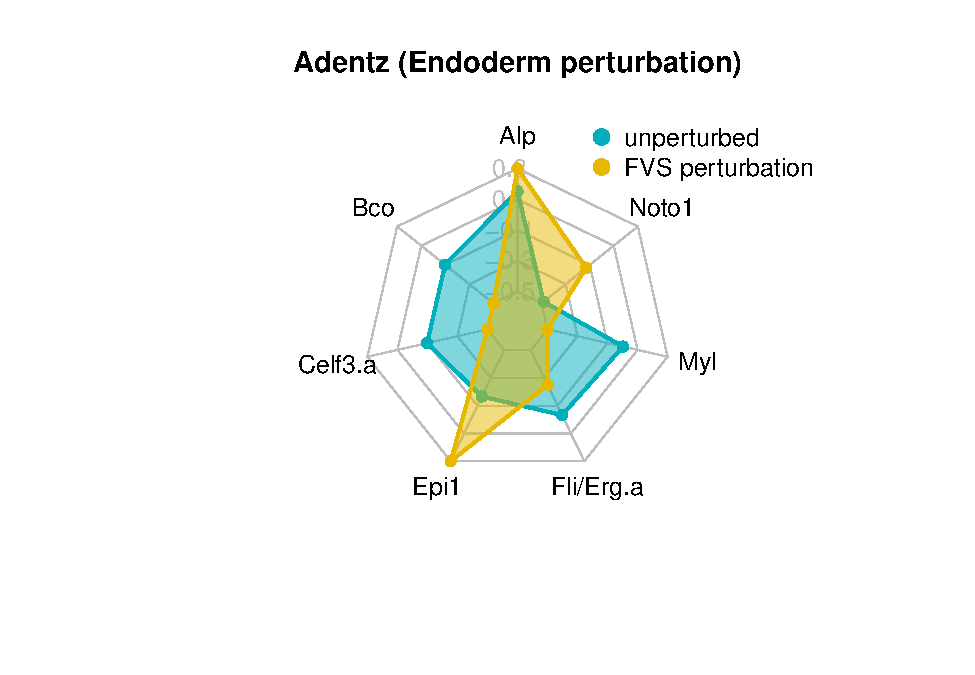
\includegraphics{_main_files/figure-latex/ascidian embryo radar plots-1.pdf} 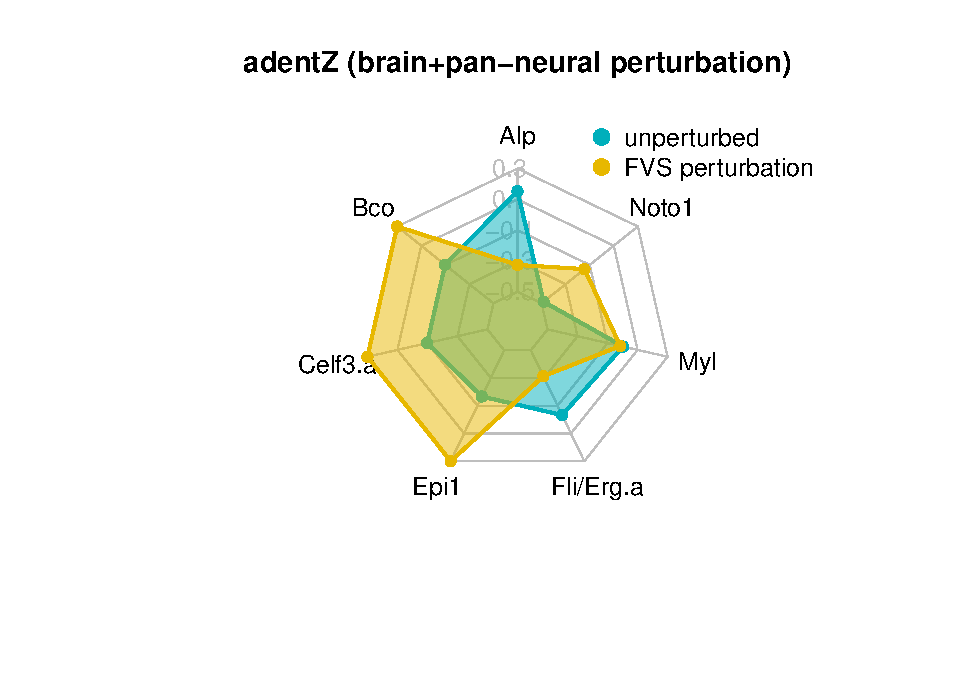
\includegraphics{_main_files/figure-latex/ascidian embryo radar plots-2.pdf} 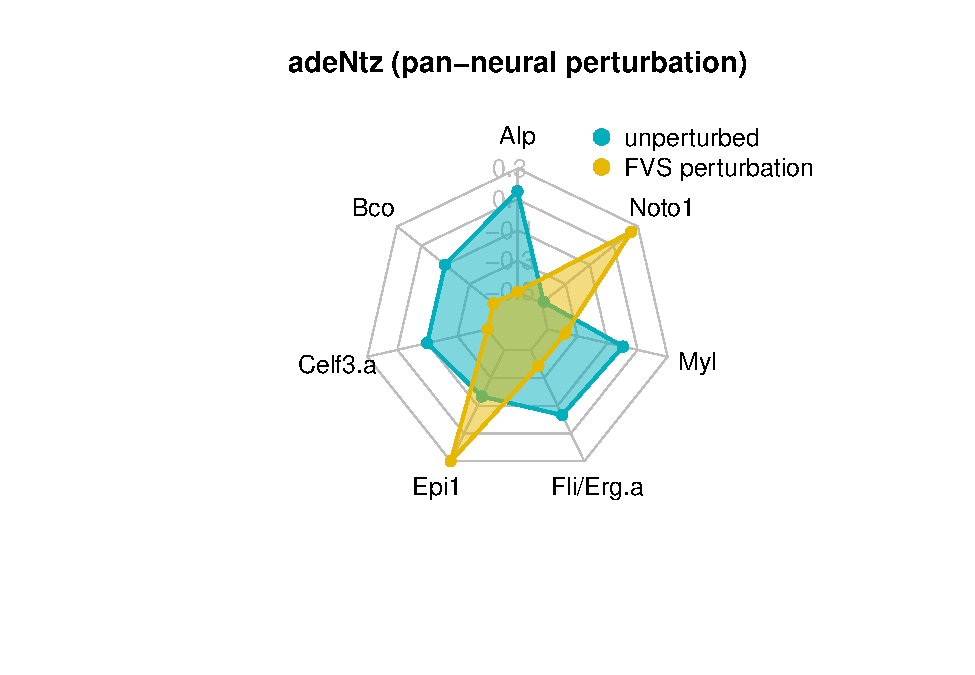
\includegraphics{_main_files/figure-latex/ascidian embryo radar plots-3.pdf} 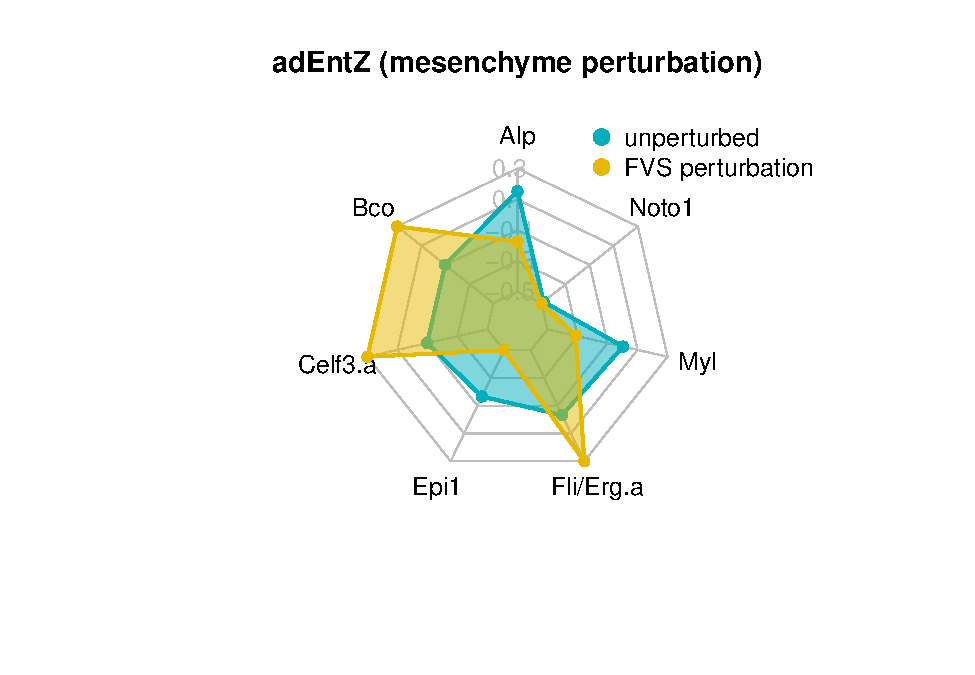
\includegraphics{_main_files/figure-latex/ascidian embryo radar plots-4.pdf} 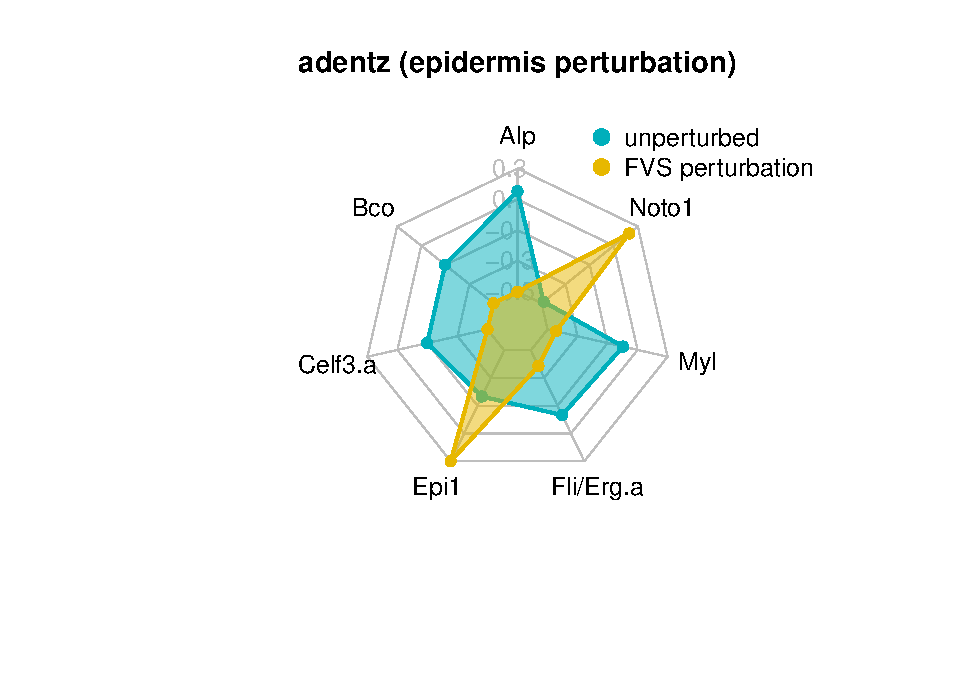
\includegraphics{_main_files/figure-latex/ascidian embryo radar plots-5.pdf} 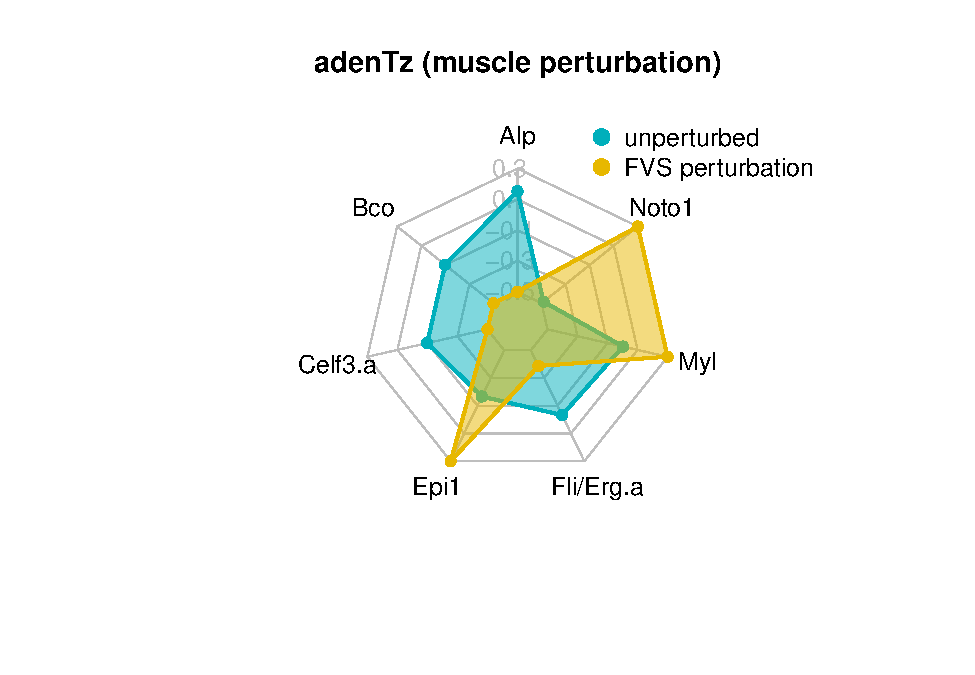
\includegraphics{_main_files/figure-latex/ascidian embryo radar plots-6.pdf} 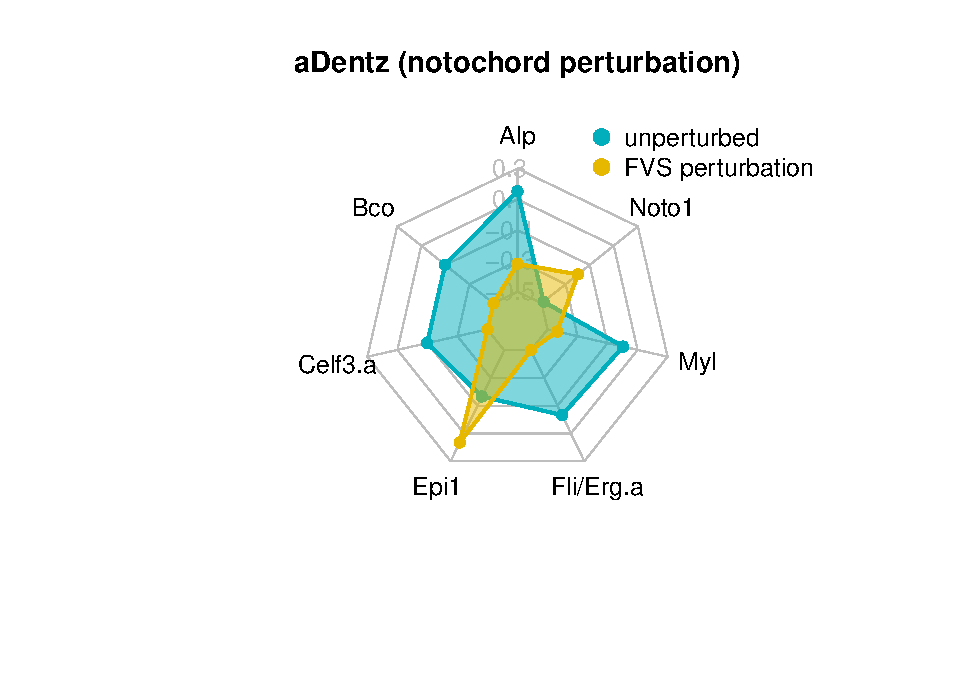
\includegraphics{_main_files/figure-latex/ascidian embryo radar plots-7.pdf}

\hypertarget{pluripotent-stem-cell-example}{%
\chapter{Pluripotent Stem Cell Example}\label{pluripotent-stem-cell-example}}

\hypertarget{adaptive-resistance-in-colorectal-cancer-example}{%
\chapter{Adaptive Resistance in Colorectal Cancer Example}\label{adaptive-resistance-in-colorectal-cancer-example}}

\hypertarget{footnotes-and-citations}{%
\chapter{Footnotes and citations}\label{footnotes-and-citations}}

\hypertarget{footnotes}{%
\section{Footnotes}\label{footnotes}}

Footnotes are put inside the square brackets after a caret \texttt{\^{}{[}{]}}. Like this one \footnote{This is a footnote.}.

\hypertarget{citations}{%
\section{Citations}\label{citations}}

Reference items in your bibliography file(s) using \texttt{@key}.

For example, we are using the \textbf{bookdown} package \citep{R-bookdown} (check out the last code chunk in index.Rmd to see how this citation key was added) in this sample book, which was built on top of R Markdown and \textbf{knitr} \citep{xie2015} (this citation was added manually in an external file book.bib).
Note that the \texttt{.bib} files need to be listed in the index.Rmd with the YAML \texttt{bibliography} key.

The RStudio Visual Markdown Editor can also make it easier to insert citations: \url{https://rstudio.github.io/visual-markdown-editing/\#/citations}

\hypertarget{blocks}{%
\chapter{Blocks}\label{blocks}}

\hypertarget{equations}{%
\section{Equations}\label{equations}}

Here is an equation.

\begin{equation} 
  f\left(k\right) = \binom{n}{k} p^k\left(1-p\right)^{n-k}
  \label{eq:binom}
\end{equation}

You may refer to using \texttt{\textbackslash{}@ref(eq:binom)}, like see Equation \eqref{eq:binom}.

\hypertarget{theorems-and-proofs}{%
\section{Theorems and proofs}\label{theorems-and-proofs}}

Labeled theorems can be referenced in text using \texttt{\textbackslash{}@ref(thm:tri)}, for example, check out this smart theorem \ref{thm:tri}.

\begin{theorem}
\protect\hypertarget{thm:tri}{}\label{thm:tri}For a right triangle, if \(c\) denotes the \emph{length} of the hypotenuse
and \(a\) and \(b\) denote the lengths of the \textbf{other} two sides, we have
\[a^2 + b^2 = c^2\]
\end{theorem}

Read more here \url{https://bookdown.org/yihui/bookdown/markdown-extensions-by-bookdown.html}.

\hypertarget{callout-blocks}{%
\section{Callout blocks}\label{callout-blocks}}

The R Markdown Cookbook provides more help on how to use custom blocks to design your own callouts: \url{https://bookdown.org/yihui/rmarkdown-cookbook/custom-blocks.html}

\hypertarget{sharing-your-book}{%
\chapter{Sharing your book}\label{sharing-your-book}}

\hypertarget{publishing}{%
\section{Publishing}\label{publishing}}

HTML books can be published online, see: \url{https://bookdown.org/yihui/bookdown/publishing.html}

\hypertarget{pages}{%
\section{404 pages}\label{pages}}

By default, users will be directed to a 404 page if they try to access a webpage that cannot be found. If you'd like to customize your 404 page instead of using the default, you may add either a \texttt{\_404.Rmd} or \texttt{\_404.md} file to your project root and use code and/or Markdown syntax.

\hypertarget{metadata-for-sharing}{%
\section{Metadata for sharing}\label{metadata-for-sharing}}

Bookdown HTML books will provide HTML metadata for social sharing on platforms like Twitter, Facebook, and LinkedIn, using information you provide in the \texttt{index.Rmd} YAML. To setup, set the \texttt{url} for your book and the path to your \texttt{cover-image} file. Your book's \texttt{title} and \texttt{description} are also used.

This \texttt{gitbook} uses the same social sharing data across all chapters in your book- all links shared will look the same.

Specify your book's source repository on GitHub using the \texttt{edit} key under the configuration options in the \texttt{\_output.yml} file, which allows users to suggest an edit by linking to a chapter's source file.

Read more about the features of this output format here:

\url{https://pkgs.rstudio.com/bookdown/reference/gitbook.html}

Or use:

\begin{Shaded}
\begin{Highlighting}[]
\NormalTok{?bookdown}\OperatorTok{::}\NormalTok{gitbook}
\end{Highlighting}
\end{Shaded}

  \bibliography{book.bib,packages.bib}

\end{document}
